\documentclass[a4paper,12pt]{article} % добавить leqno в [] для нумерации слева
\usepackage[a4paper,top=1.3cm,bottom=2cm,left=1.5cm,right=1.5cm,marginparwidth=0.75cm]{geometry}
%%% Работа с русским языком
\usepackage{cmap}					% поиск в PDF
\usepackage[warn]{mathtext} 		% русские буквы в фомулах
\usepackage[T2A]{fontenc}			% кодировка
\usepackage[utf8]{inputenc}			% кодировка исходного текста
\usepackage[english,russian]{babel}	% локализация и переносы
\usepackage{physics}
\usepackage{multirow}
\usepackage{bm}
\usepackage{longtable}

%%% Нормальное размещение таблиц (писать [H] в окружении таблицы)
\usepackage{float}
\restylefloat{table}


\usepackage{graphicx}

\usepackage{wrapfig}
\usepackage{tabularx}

\usepackage{hyperref}
\usepackage[rgb]{xcolor}
\hypersetup{
	colorlinks=true,urlcolor=blue
}
\usepackage{pgfplots}
\pgfplotsset{compat=1.9}
%%% Дополнительная работа с математикой
\usepackage{amsmath,amsfonts,amssymb,amsthm,mathtools} % AMS
\usepackage{icomma} % "Умная" запятая: $0,2$ --- число, $0, 2$ --- перечисление

%% Номера формул
%\mathtoolsset{showonlyrefs=true} % Показывать номера только у тех формул, на которые есть \eqref{} в тексте,

%% Шрифты
\usepackage{euscript}	 % Шрифт Евклид
\usepackage{mathrsfs} % Красивый матшрифт

%% Свои команды
\DeclareMathOperator{\sgn}{\mathop{sgn}}

%% Перенос знаков в формулах (по Львовскому)
%\newcommand*{\hm}[1]{#1\nobreak\discretionary{}
%	{\hbox{$\mathsurround=0pt #1$}}{}}

\date{\today}

\begin{document}

\begin{titlepage}
	\begin{center}
		{\large МОСКОВСКИЙ ФИЗИКО-ТЕХНИЧЕСКИЙ ИНСТИТУТ (НАЦИОНАЛЬНЫЙ ИССЛЕДОВАТЕЛЬСКИЙ УНИВЕРСИТЕТ)}
	\end{center}
	\begin{center}
		{\large Физтех-школа физики и исследований им. Ландау}
	\end{center}
	
	
	\vspace{4.5cm}
	{\huge
		\begin{center}
			{\bf Отчёт о выполнении лабораторной работы №3.4.5}\\
			Петля Гистерезиса (динамический метод)
		\end{center}
	}
	\vspace{2cm}
	\begin{flushright}
		{\LARGE Автор:\\ Сенокосов Арсений Олегович \\
			\vspace{0.2cm}
			Б02-012}
	\end{flushright}
	\vspace{8cm}
	\begin{center}
		Долгопрудный\\
		\today
	\end{center}
\end{titlepage}
%\numberwithin{equation}{section}

\section{Введение}

\textbf{Цель работы:} изучение петель гистерезиса различных ферромагнитных
материалов в переменных полях.

\textbf{В работе используются:} автотрансформатор, понижающий трансформатор, интегрирующая цепочка, амперметр, вольтметр, электронный
осциллограф, делитель напряжения, тороидальные образцы с двумя обмотками.


\section{Теоретические сведения}

Основные характеристики
ферромагнетиков — их коэрцитивное поле $H_c$, магнитная проницаемость
$\mu$, рассеиваемая в виде тепла при перемагничивании мощность — зависят
от частоты перемагничивающего поля. В данной работе кривые гистерезиса ферромагнитных материалов изучаются в поле частоты $\nu_0 =$ 50 Гц
с помощью электронного осциллографа.
\begin{figure}[H]
	\centering
	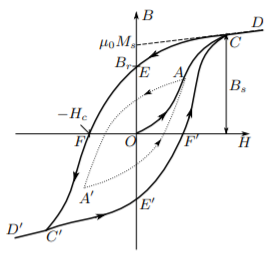
\includegraphics{petlya.png}
	\caption{Петля гистерезиса ферромагнетика}
	\label{fig:petlya}
\end{figure}

Магнитная индукция $ B $ и напряжённость поля $ H $ в ферромагнитном материале неоднозначно связаны между собой: индукция зависит
не только от напряжённости, но и от предыстории образца. Связь между $ B $ и $ H $ типичного ферромагнетика иллюстрирует рис. $\ref{fig:petlya}$.

Если к ферромагнитному образцу прикладывать переменное внешнее
магнитное поле, то его состояние на плоскости $ B-H $ будет изменяться
по замкнутой кривой — петле гистерезиса. Размер петли определяется
максимальным значением напряжённости $ H $ в цикле (например, петля $ AA' $,
обозначенная пунктиром на рис. $\ref{fig:petlya}$). Если амплитуда напряжённости достаточно велика, то образец будет периодически достигать насыщения,
что на рисунке соответствует кривой $ CEFC'E'F'C $ (предельная петля
гистерезиса). Пересечение предельной петли с вертикальной осью соответствует остаточной индукции $B_r$, пересечение с горизонтальной осью
— коэрцитивному полю $H_c$. Крайние точки петель, соответствующие амплитудным значениям $ H $ (например, точка $ A $ на рис. $\ref{fig:petlya}$), лежат на начальной кривой намагничивания ($ OAC $).

\textbf{Измерение магнитной индукции.} Магнитную индукцию $ B $ удобно
определять с помощью ЭДС, возникающей при изменении магнитного
потока $ \Phi $ в катушке, намотанной на образец. Пусть катушка c $ N $ витками плотно охватывает образец сечением $ S $, и индукция $ B $ в образце
однородна. Тогда

\begin{equation}
|B|=\frac{1}{SN}\int\mathcal{E} dt.
\label{eq:|B|}
\end{equation}
\begin{wrapfigure}{r}{0.35\linewidth}
	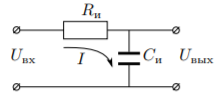
\includegraphics[width=\linewidth]{int.png}
	\caption{Интегрирующая ячейка}
	\label{fig:int}
\end{wrapfigure}

Для интегрирования в работе используется интегрирующая $ RC $-цепочка (рис. $ \ref{fig:int} $).
«Входное» напряжение от источника $U_{\text{вх}}(t)$ подаётся на последовательно соединённые резистор $R_\text{и}$ и конденсатор $C_\text{и}$. <<Выходное>>
напряжение $U_{\text{вых}}(t)$ снимается с конденсатора. Предположим, что 1) сопротивление источника мало по сравнению с $R_\text{и}$, 2) выходное сопротивление (сопротивление на входе осциллографа), напротив, велико: $R_{\text{вых}}$ $ \gg $ $R_\text{и}$ и, наконец, 3) сопротивление $R_\text{и}$ достаточно велико, так что почти всё падение напряжения приходится на него, а $U_{\text{вых}}$ $\ll$ $U_{\text{вх}}$. В таком случае ток цепи равен I = ($U_{\text{вх}}$ - $U_{\text{вых}}$)/$R_\text{и}$ $\approx$ $U_{\text{вх}}$/$R_\text{и}$, и входное и выходное сопротивление связаны соотношением
\begin{equation}
U_{\text{вых}} = \frac{q}{C_\text{и}} = \frac{1}{C_\text{и}}\int\limits_0^t Idt \approx \frac{1}{\tau_\text{и}} \int\limits_0^t U_{\text{вх}}dt,
\label{eq:U_ext}
\end{equation}
где $\tau_\text{и}=R_\text{и}C_\text{и}$ - постоянная времени $ RC $ - цепочки. Для индукции поля из ($\ref{eq:|B|}$) получаем 
\begin{equation}
|B|=\frac{1}{SN}\int U_{\text{вх}} dt=\frac{\tau_\text{и}}{SN}U_{\text{вых}}.
\label{eq:|B|new}
\end{equation}

\textbf{Замечание.} Уточним критерий применимости соотношения ($\ref{eq:U_ext}$). Пусть на вход интегрирующей ячейки подан синусоидальный сигнал с частотой $\omega_0$. Тогда, пользуясь методом комплексных амплитуд, нетрудно найти отношение амплитуд входного и выходного напряжений:
\begin{equation}
\frac{U_{\text{вых}}}{U_{\text{вх}}}=\frac{1/\omega_0C}{\sqrt{R^2+1/(\omega_0C)^2}}.
\end{equation}
Тогда неравенство $U_{\text{вых}} \ll U_{\text{вх}}$ реализуется, если 
\begin{equation}
\tau \equiv RC\gg \frac{1}{\omega_0}
\end{equation}
(импеданс конденсатора мал по сравнению сопротивлением резистора).
В таком случае для синусоидального сигнала имеем
\begin{equation}
\frac{U_{\text{вых}}}{U_{\text{вх}}}\approx\frac{1}{\omega_0\tau}.
\end{equation}
В общем случае, если $\omega_0$ — частота самой низкой гармоники в спектре
произвольного входного сигнала, то при $\omega_0\tau \gg 1$ неравенство $U_{\text{вых}} \ll U_{\text{вх}}$ выполняется на любой частоте $\omega > \omega_0$.


\section{Экспериментальная установка}

Схема установки изображена на рис. $\ref{fig:scheme}$. Напряжение сети (220 В,
50 Гц) с помощью трансформаторного блока Т, состоящего из регулировочного автотрансформатора и разделительного понижающего трансформатора, подаётся на намагничивающую обмотку $N_0$ исследуемого образца.
\begin{figure}[h!]
	\centering
	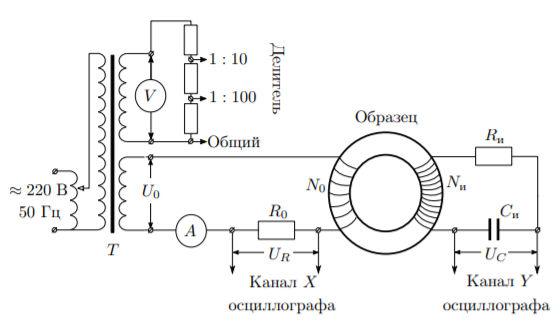
\includegraphics{scheme.png}
	\caption{ Схема установки для исследования намагничивания образцов}
	\label{fig:scheme}
\end{figure}

В цепь намагничивающей катушки, на которую подаётся некоторое
напряжение $U_0$, последовательно включено сопротивление $R_0$. Напряжение на $R_0$, равное $U_R$= $R_0I_0$, где $I_0$ — ток в намагничивающей обмотке $N_0$, подаётся на канал $ X $ осциллографа. Связь напряжённости $ H $ в
образце и тока $I_0$ рассчитывается по теореме о циркуляции. 
Действующее значение переменного тока в обмотке $N_0$ измеряется амперметром A.
Для измерения магнитной индукции $ B $ с измерительной обмотки $N_\text{и}$
на вход $ RC $-цепочки подаётся напряжение $U_\text{и}$ ($U_{\text{вх}}$), пропорциональное
производной $ dB/dt $. С интегрирующей ёмкости $C_\text{и}$ снимается напряжение $U_C$ ($U_{\text{вых}}$), пропорциональное величине $ B $, и подаётся на вход $ Y $
осциллографа. Значение индукции поля $ B $ рассчитывается по формуле ($\ref{eq:|B|new}$).
Замкнутая кривая, возникающая на экране, воспроизводит в некотором масштабе (различном для осей $ X $ и $ Y $) петлю гистерезиса. Чтобы придать этой кривой количественный смысл, необходимо установить
масштабы изображения, т. е. провести калибровку каналов $ X $ и $ Y $ осциллографа.

\section{Ход работы}
\subsection{Измерение петель гистерезиса}

Соберем схему согласно рис. $\ref{fig:scheme}$. Подберем ток питания в намагничивающей обмотке с помощью автотрансформатора и коэффициенты усиления ЭО таким образом, чтобы предельная петля гистерезиса занимала большую часть экрана. Приведем характерные значения катушек разных материалов в таблице \ref{tab:har_kat}.

\begin{table}[H]
	\centering
	\begin{tabular}{|c|c|c|c|c|}
		\hline
		Материал     & $N_0$ & $N_\text{и}$ & $S^2$, см$^2$ & $2\pi R$, см \\ \hline
		Феррит       & 40    & 400                              & 3,0           & 25,0         \\ \hline
		Пермаллой    & 20    & 300                              & 0,8           & 13,3         \\ \hline
		Крем. железо & 25    & 250                              & 2,0           & 11,0         \\ \hline
	\end{tabular}
	\caption{Характеристики катушек}
	\label{tab:har_kat}
\end{table}

Для каждого образца получим передельные петли гистерезиса, по коэффициентам усиления ЭО $K_x$ и $K_y$ рассчитаем масштабы, определим двойные амплитуды коэрцетивной силы $ [2x(c)] $ и индукции насыщения $ [2y(s)] $. Масштабы по осям $ X $ и $ Y $ рассчитаем по формулам 
$H=IN_0/(2\pi R),\ где\ I=K_x/R_0;\ B=R_\text{и}C_\text{и}U_{\text{вых}}/(SN_\text{и}),$ где $U_{\text{вых}}=K_y$. Результаты измерений и вычислений занесём в таблицу \ref{tab:izm}.

\begin{table}[H]
	\centering
	\begin{tabular}{|c|c|c|c|c|}
		\hline
		Материал     & $[2x(c)]$, дел & $[2y(s)]$, дел & $K_x$, мВ/дел & $K_y$, мВ/дел \\ \hline
		Феррит       & 1,0            & 4,8            & 20            & 20            \\ \hline
		Пермаллой    & 3,6            & 3,6            & 20            & 50            \\ \hline
		Крем. железо & 1,2            & 4,4            & 100           & 50            \\ \hline
	\end{tabular}
\end{table}

\begin{table}[H]
	\centering
	\begin{tabular}{|c|c|c|c|}
		\hline
		Материал     & $I_\text{эфф}$, мА & $H$, А$\cdot$м$^{-1}$ / дел & $B$, Тл/дел \\ \hline
		Феррит       & 215                & 14,5                        & 0,07        \\ \hline
		Пермаллой    & 165                & 13,7                        & 0,88        \\ \hline
		Крем. железо & 238                & 103,3                       & 0,40        \\ \hline
	\end{tabular}
	\caption{Результаты измерений}
	\label{tab:izm}
\end{table}

Теперь, зная масштабы по осям, можно определить значения коэрцетивной силы $ H_c $
и индукции насыщения $ B_s $. Результаты заносим в таблицу \ref{tab:vichisl}.

\begin{table}[H]
	\centering
	\begin{tabular}{|c|c|c|c|c|}
		\hline
		Материал     & $H_c$, А/м & $\sigma_{H_c}$, А/м & $B_s$, Тл & $\sigma_{B_s}$, Тл \\ \hline
		Феррит       & 7,27       & 0,76                & 0,16      & 0,01               \\ \hline
		Пермаллой    & 24,61      & 2,20                & 1,58      & 0,13               \\ \hline
		Крем. железо & 61,98      & 7,30                & 0,88      & 0,06               \\ \hline
	\end{tabular}
	\caption{Результаты вычислений}
	\label{tab:vichisl}
\end{table}

Также в следующую таблицу \ref{tab:tab} занесём табличные данные для значений коэрцетивной силы $ H_c $ и индукции насыщения $ B_s $.

\begin{table}[H]
	\centering
	\begin{tabular}{|c|c|c|}
		\hline
		Материал     & $H_c$, А/м & $B_s$, Тл \\ \hline
		Феррит       & 20         & 0,27      \\ \hline
		Пермаллой    & 11--40     & 1,51      \\ \hline
		Крем. железо & 50--100    & 1,21      \\ \hline
	\end{tabular}
	\caption{Табличные данные}
	\label{tab:tab}
\end{table}

Сравнивая полученные данные с табличными можно утверждать, что они совпадают, по крайней мере по порядку величины. Также приведём фотографии предельных петель гистерезиса.

\begin{figure}[h!]
	\centering
	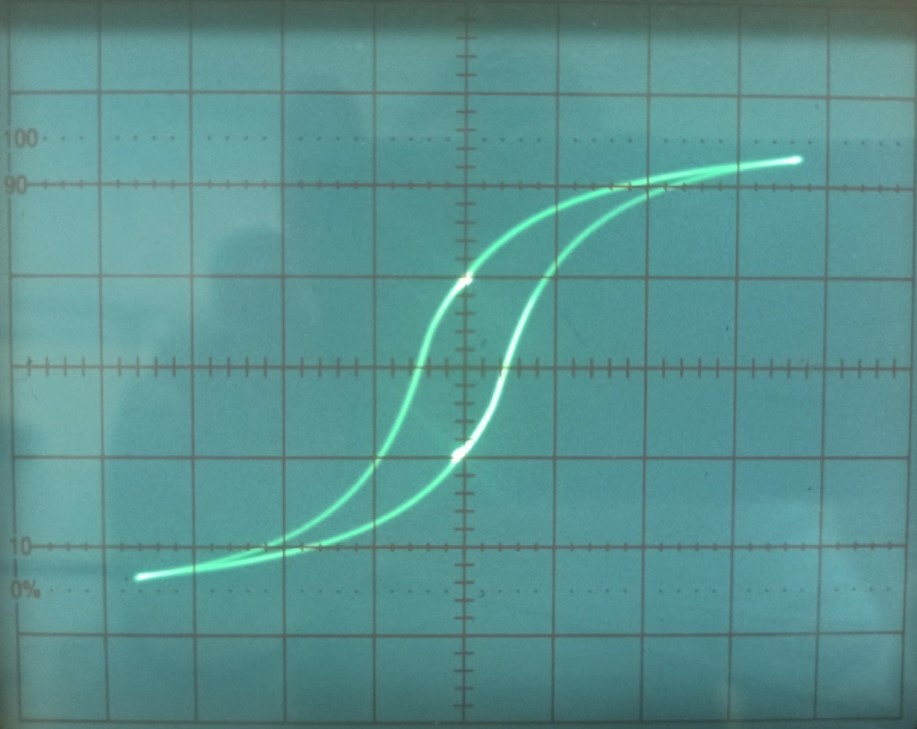
\includegraphics[width=8cm]{ferrit.jpg}
	\caption{Предельная петля гистерезиса феррита}
\end{figure}
\begin{figure}[h!]
	\centering
	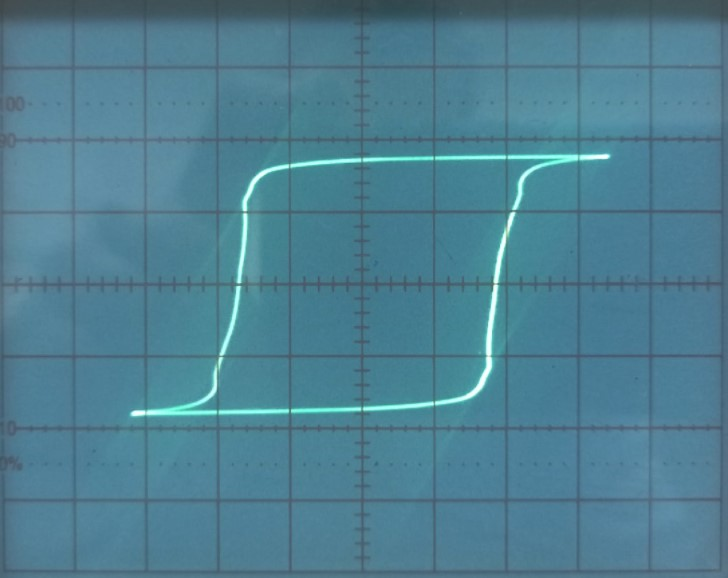
\includegraphics[width=8cm]{permalloi.jpg}
	\caption{Предельная петля гистерезиса пермаллоя}
\end{figure}
\newpage
\begin{figure}[h!]
	\centering
	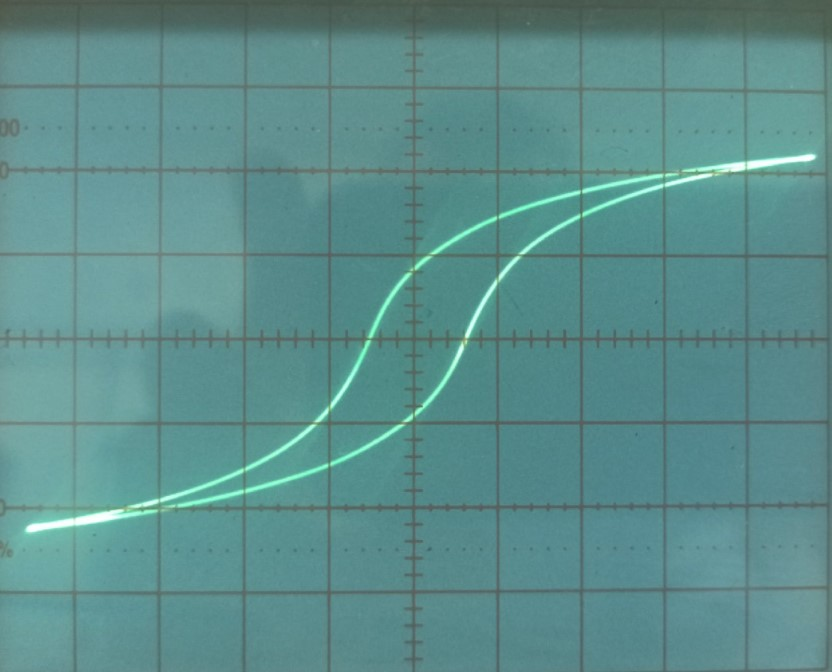
\includegraphics[width=8cm]{Si_Fe.jpg}
	\caption{Предельная петля гистерезиса для кремнистого железа}
\end{figure}

\subsection{Проверка калибровки осциллографа}

Проверим калибровку ЭО по оси X. Отключим намагничивающую обмотку $N_0$ от цепи, соединив оба провода, идущих к обмотке, на одной ее клемме. С помощью автотрансформатора подберем такой ток через $R_0$, при котором горизонтальная прямая занимает большую часть экрана. При $ K_x=0,1 \text{ В/дел} $ рассчитаем чувствительность $m_x=0,097 \text{ В/дел}$.

Аналогичные действия проводим при $ K_x =0,02 \text{ В/дел} $. Получаем $ m_x=0,019 \text{ В/дел} $.

Так как $m_x \approx K_x$, ЭО откалиброван по оси X корректно.

Также необходимо проверить калибровку по оси $ Y $. Для этого соединим вход Y ЭО с клеммам делителя "1:100 - земля". Не меняя рабочего коэффициента $K_y = 0,05\text{ В/дел}$, подберем с помощью трансформатора напряжение, при котором вертикальная прямая занимает большую часть экрана. Подключим вольтметр V к тем же клеммам делителя и, используя измеренное $U_{\text{эф}}$, рассчитаем чувствительность $m_y=0,048\text{ В/дел}$.

Те же действия повторяем при $K_y = 0,02\text{ В/дел}$. Получаем $m_y=0,017\text{ В/дел}$.

Так как $m_y \approx K_y$, ЭО откалиброван по оси Y корректно.

\subsection{Проверка применимости теоретических выкладок}

Проверим применимость формулы ($\ref{eq:U_ext}$). Для этого рассчитаем $\tau$ -- постоянную времени $ RC $-цепочки. Для определения напряжений на входе и выходе интегрирующей ячейки соединим вход ячейки с обмоткой <<6,3 В>> трансформатора. Подключим Y-вход ЭО ко входу интегрирующей ячейки и отключим X-вход ЭО. Подберем такой ток, чтобы вертикальная прямая занимала большую часть экрана, и определим входное напряжение $U_{\text{вх}}=2y\cdot K_y=6,8\ \text{дел} \cdot 2\ \text{В/дел}=13,6\ \text{В}$. Не меняя тока, подключим Y-вход ЭО к выходу ячейки и аналогичным образом определим $U_{\text{вых}}=2y\cdot K_y=5,2\ \text{дел} \cdot 0,02\ \text{В/дел}=0,104\ \text{В}$. Рассчитаем $\tau=\frac{U_{\text{вх}}}{\omega U_{\text{вых}}}=\frac{13,6}{0,104\cdot2\pi\cdot 50}=0,416\ \text{c}$, где $\omega=2\pi\nu$. По определению $\tau_{RC}=R_\text{и}C_\text{и}=0,4\ \text{с}$. Так как $\tau\approx\tau_{RC}$, то условия применимости нашей теории выполнены.

\subsection{Обсуждение результатов и выводы}

В ходе выполнения данной лабораторной работы были исследованы петли гистерезиса для трех различных образцов и получены характерные величины для каждого образца, которые сошлись с табличными значениями по порядку величины. Кроме того, была проверена применимость используемого метода в условиях нашего эксперимента. В итоге было установлено, что условия применимости выполняются и метод является неплохим способом определения характерных параметров для ферромагнитных материалов.




\end{document}